% =============================================================================
% Trained AI-code detectors key on formatting, not authorship — research report.
% EDIT THIS FILE BY HAND. Prose lives here. Every NUMBER is a \res... macro
% defined in macros.tex (auto-generated by scripts/06_build_macros.py).
% Citations come from refs.bib (auto-generated by scripts/build_bib.py from
% refs_ids.toml) — never hand-type bib metadata.
% Build:  cd paper && latexmk -pdf paper.tex
% =============================================================================
\documentclass[11pt]{article}
\usepackage[margin=1in]{geometry}
\usepackage{graphicx}
\usepackage{booktabs}
\usepackage{amsmath}
\usepackage{xcolor}
\usepackage[numbers,sort&compress]{natbib}
\usepackage[hidelinks]{hyperref}
\graphicspath{{../results/figures/}}
% AUTO-GENERATED by scripts/06_build_macros.py from results/analysis.json.
% Variables only. Do NOT edit by hand and do NOT type numbers into paper.tex —
% reference these macros (\res...) instead. Re-run the pipeline to refresh.
\newcommand{\resAtHiLoBinoculars}{-0.39}
\newcommand{\resAtHiLoDroidDetect}{-0.37}
\newcommand{\resAtHiLoFastDetectGPT}{-1.00}
\newcommand{\resAtNHighSkill}{9}
\newcommand{\resAtNLowSkill}{45}
\newcommand{\resAtRatingHighSkill}{2225}
\newcommand{\resAtRatingLowSkill}{323}
\newcommand{\resAtSlopeBinoculars}{-0.043}
\newcommand{\resAtSlopeDroidDetect}{-0.100}
\newcommand{\resAtSlopeFastDetectGPT}{-0.167}
\newcommand{\resAurocMatchedBinoculars}{0.665}
\newcommand{\resAurocMatchedDroidDetect}{0.741}
\newcommand{\resAurocMatchedFastDetectGPT}{0.704}
\newcommand{\resAurocMismatchedBinoculars}{0.667}
\newcommand{\resAurocMismatchedDroidDetect}{0.752}
\newcommand{\resAurocMismatchedFastDetectGPT}{0.700}
\newcommand{\resDeltaBinoculars}{0.002}
\newcommand{\resDeltaCIhiBinoculars}{0.006}
\newcommand{\resDeltaCIhiDroidDetect}{0.021}
\newcommand{\resDeltaCIhiFastDetectGPT}{-0.000}
\newcommand{\resDeltaCIloBinoculars}{-0.002}
\newcommand{\resDeltaCIloDroidDetect}{0.002}
\newcommand{\resDeltaCIloFastDetectGPT}{-0.009}
\newcommand{\resDeltaDroidDetect}{0.011}
\newcommand{\resDeltaFastDetectGPT}{-0.004}
\newcommand{\resHumanSlopeBinoculars}{0.07}
\newcommand{\resHumanSlopeDroidDetect}{-0.29}
\newcommand{\resHumanSlopeFastDetectGPT}{-0.30}
\newcommand{\resHumanSlopeHiBinoculars}{0.34}
\newcommand{\resHumanSlopeHiDroidDetect}{-0.06}
\newcommand{\resHumanSlopeHiFastDetectGPT}{-0.12}
\newcommand{\resHumanSlopeLoBinoculars}{-0.21}
\newcommand{\resHumanSlopeLoDroidDetect}{-0.52}
\newcommand{\resHumanSlopeLoFastDetectGPT}{-0.46}
\newcommand{\resLegAuthorCPythonCore}{0.875}
\newcommand{\resLegAuthorCPythonCoreN}{40}
\newcommand{\resLegAuthorDRichardHipp}{0.275}
\newcommand{\resLegAuthorDRichardHippN}{40}
\newcommand{\resLegAuthorLinusTorvalds}{0.400}
\newcommand{\resLegAuthorLinusTorvaldsN}{15}
\newcommand{\resLegAuthorSalvatoreSanfilippo}{0.350}
\newcommand{\resLegAuthorSalvatoreSanfilippoN}{40}
\newcommand{\resLegFlagBinoculars}{0.200}
\newcommand{\resLegFlagDroidDetect}{0.489}
\newcommand{\resLegFlagDroidNative}{0.785}
\newcommand{\resLegFlagFastDetectGPT}{0.126}
\newcommand{\resLlmSlopeBinoculars}{-0.19}
\newcommand{\resLlmSlopeDroidDetect}{-0.09}
\newcommand{\resLlmSlopeFastDetectGPT}{-0.54}
\newcommand{\resLlmSlopeHiBinoculars}{-0.14}
\newcommand{\resLlmSlopeHiDroidDetect}{-0.05}
\newcommand{\resLlmSlopeHiFastDetectGPT}{-0.50}
\newcommand{\resLlmSlopeLoBinoculars}{-0.24}
\newcommand{\resLlmSlopeLoDroidDetect}{-0.14}
\newcommand{\resLlmSlopeLoFastDetectGPT}{-0.59}
\newcommand{\resMeanDelta}{0.003}
\newcommand{\resMeanHumanSlope}{-0.17}
\newcommand{\resNAtcoder}{54}
\newcommand{\resNCf}{2655}
\newcommand{\resNLegendary}{135}
\newcommand{\resNModels}{3}
\newcommand{\resStyleCommentDensityEasy}{0.021}
\newcommand{\resStyleCommentDensityHard}{0.028}
\newcommand{\resStyleHasTypeHintsEasy}{0.594}
\newcommand{\resStyleHasTypeHintsHard}{0.755}
\newcommand{\resStyleMeanIdentifierLenEasy}{2.724}
\newcommand{\resStyleMeanIdentifierLenHard}{2.482}
\newcommand{\resStyleRsqBinoculars}{0.071}
\newcommand{\resStyleRsqDroidDetect}{0.128}
\newcommand{\resStyleRsqFastDetectGPT}{0.276}


\newcommand{\skillaxis}{competitive-programming difficulty}
\title{Trained AI-Code Detectors Key on \emph{Formatting}, Not Authorship\\
\large A semantics-preserving red-team of DroidDetect (and a null skill confound)}
\author{Autonomous experiment (Claude Code) for Matthew}
\date{\today}

\begin{document}
\maketitle

\begin{center}
\fcolorbox{red!70!black}{red!5}{\parbox{0.92\linewidth}{\centering
\textbf{\textcolor{red!70!black}{Done by AI, not verified by human.}}
This report was produced \emph{autonomously} by an AI agent (Claude Code). Its experiments,
numbers, figures, and prose have \emph{not} been checked by a human. Treat every result and
claim as provisional and independently verify before citing or relying on it.}}
\end{center}
\vspace{0.5em}

\begin{abstract}
We set out to ask whether AI-code detectors track author \textbf{species} (human vs.\ LLM)
or author \textbf{skill/style}, and arrived at a sharper, more cautionary answer about the one
family of off-the-shelf trained code detectors we could obtain.
\textbf{(1) Headline.} DroidDetect~\citep{orel2025droid}, a ModernBERT-based~\citep{warner2024modernbert}
detector that we load faithfully---reproducing the authors' performance on their \emph{own}
DroidCollection Python test data (AUROC \resDroidInDistAUROC{}, \resDroidInDistHumanFPR{} human
false-positive rate)---has its verdict \emph{flipped} by a \emph{semantics-preserving}
reformatting. Running its own human test code through \texttt{black}~\citep{langa2020black} (the
standard formatter, which keeps comments and only restyles layout) raises the fraction it calls
``machine'' from \textbf{\resAblDcHumanOrig{}} to \textbf{\resAblDcHumanBlack{}}
(\texttt{ast.unparse} gives \resAblDcHumanCanon{}), collapsing the human/machine separation from
\resAblGapOrig{} to \resAblGapBlack{}. Stripping comments \emph{alone} barely moves it
(\resAblDcHumanStrip{}); identifiers, literals, and docstrings are preserved exactly. The
operative signal is therefore layout/quote/wrap style, not authorship and not lexical content.
This is consistent with a data-collection artifact (machine code is born auto-formatted, human
code is scraped as-is) and a shortcut-learning failure~\citep{geirhos2020shortcut}, and it
reproduces across \emph{every} sibling in the family (Sec.~\ref{sec:family}).
\textbf{(2) Consequence.} This formatting dependence explains a dramatic cross-source failure:
on tidy human Codeforces Python from a \emph{different} scrape~\citep{matrixstudio2024codeforces}
the same model labels \resDroidArgmaxCfHumanFPR{} of ordinary human code AI, and
\resDroidArgmaxLegendary{} of contamination-free pre-LLM elite code (Torvalds' \texttt{git},
antirez's Redis, Hipp's SQLite, CPython)---at roughly its own false-positive rate, i.e.\ a
domain-shift over-flagging, not an ``elite-code'' effect.
\textbf{(3) Skill.} On the \skillaxis{} axis we find a \emph{null}: the skill confound is bounded
small ($\Delta_{\text{confound}}\!\approx\!\resMeanDelta{}$, 95\% CI upper bound
\resDeltaCIhiDroidDetect{} AUROC for the trained detector), with within-species slopes that do not
support a skill-tracking account. \textbf{Deployment implication:} an integrity tool calibrated on
one corpus can flag the majority of \emph{legitimate} human code simply because the author ran a
code formatter---a false-positive failure mode invisible to the i.i.d., fixed-threshold-free
accuracy such tools report. The zero-shot statistical detectors~\citep{bao2023fastdetectgpt,hans2024binoculars}
do not collapse this way, but are near-random on this domain---all three detectors fail here,
differently.
\end{abstract}

\section{Question and hypotheses}
Post-RLHF code models are tuned toward idiomatic, well-structured ``senior-engineer''
style. If detectors learned that style as the AI signal, then \emph{AI-vs-human}
detection partly reduces to \emph{expert-vs-novice} detection. We pre-registered:
\begin{itemize}
  \item \textbf{H$_\text{species}$}: detectors classify species; within-species skill has
        no effect (slopes $\approx 0$; AUROC constant across skill cells).
  \item \textbf{H$_\text{skill}$}: detectors classify skill; among humans, higher skill
        $\to$ more ``AI''; among LLMs, novice prompting $\to$ less ``AI''.
  \item \textbf{H$_\text{mixed}$}: a weighted combination.
\end{itemize}
The headline finding is orthogonal to all three and emerged from a robustness check: the
trained detector keys on a surface feature (formatting) that none of the hypotheses anticipated.

\section{Background and related work}
\textbf{Zero-shot detectors} score text by its own likelihood geometry under a reference LM:
DetectGPT~\citep{mitchell2023detectgpt} via probability curvature, Fast-DetectGPT~\citep{bao2023fastdetectgpt}
via an analytic conditional-probability discrepancy, and Binoculars~\citep{hans2024binoculars} via
a cross-perplexity ratio. We use the latter two as canonical, vendored baselines.
\textbf{Trained detectors} fine-tune an encoder on a labeled human/machine corpus; DroidDetect is
trained on DroidCollection~\citep{orel2025droid} atop ModernBERT~\citep{warner2024modernbert} and
is, to our knowledge, the strongest openly released trained \emph{code} detector. We could not
locate any independent out-of-the-box trained code detector of comparable provenance to test
against; the entire family we evaluate shares these authors and this training data, which we treat
as a central limitation.
\textbf{Shortcut learning}~\citep{geirhos2020shortcut} names the failure where a classifier exploits
a spurious surface feature that is predictive in-distribution but invalid under shift. The closest
prior instance for detectors is \citet{liang2023detectors}, who show that text detectors are biased
against non-native English writers---a surface-feature false positive. Our result is the code
analog, with layout/formatting as the shortcut. Notably the DroidDetect authors report
i.i.d.\ F1 with a documented cross-domain collapse (their Table~3) but no fixed-FPR or calibration
metrics, and their attention interpretability (their \S E.2: weight on whitespace, punctuation, and
blank lines) is consistent with the formatting shortcut we isolate causally here.

\section{Data and methods}
\textbf{Human.} Accepted Python-3 Codeforces solutions~\citep{matrixstudio2024codeforces}, difficulty
bands easy ($\le 1200$) and hard ($\ge 1900$). \emph{Deviation from the original plan:} no public
dataset co-locates human source code with \emph{author} Elo, so the human skill axis is problem
difficulty---a noisy, and as it turns out stylistically inverted, proxy.
\textbf{LLM.} \resNModels{} models (gemma-2-2b-it, Qwen2.5-3B-Instruct, and the frontier
\texttt{gpt-5.4-nano}\footnote{\texttt{gpt-5.4-nano} is OpenAI's nano-tier model of the GPT-5.4
generation, accessed via the OpenAI API in May 2026.}) under natural/novice/expert prompts on the
same problems. \textbf{Detectors} (oriented higher${}={}$more AI): DroidDetect-Base-Binary
(trained)~\citep{orel2025droid}; Fast-DetectGPT~\citep{bao2023fastdetectgpt} and
Binoculars~\citep{hans2024binoculars} (statistical; canonical vendored implementations).
\textbf{Stats.} AUROC is primary (threshold-free); all CIs use a cluster bootstrap over
\emph{problems}; the within-species score slope (z-scored detector output regressed on the
skill axis) is the mechanism test; $\Delta_{\text{confound}}$ is reported per detector.
We apply no multiple-comparisons correction across the (detector $\times$ species $\times$ band)
intervals and accordingly do not lean on any single CI's exclusion of zero.

\section{Results}

\subsection{DroidDetect's verdict is gated by formatting (headline)}
\label{sec:headline}
We first establish the detector is loaded correctly: on the authors' own DroidCollection
Python test set it scores AUROC \resDroidInDistAUROC{} with a \resDroidInDistHumanFPR{}
human false-positive rate and \resDroidInDistMachineFlag{} machine recall---reproducing the
published numbers. So the behavior below is a property of the model, not a loading bug. We then
apply \emph{semantics-preserving} reformatters to the input code and re-score, using two
deliberately: \textbf{(i) \texttt{black}}, which restyles whitespace/indentation/quote-style/
line-wrapping but \emph{keeps comments and docstrings}; \textbf{(ii) \texttt{ast.unparse(ast.parse(code))}},
which additionally drops \texttt{\#} comments. Neither alters the lexical content a detector might
legitimately use---variable and function names, string/numeric literals, and docstrings are all
retained (we verify the identifier-token multiset is preserved at a mean of \resAblIdentPreserved{},
i.e.\ exactly). These are \emph{formatting} changes, not ``humans and AI use different words'' changes.

The effect is dramatic (Fig.~\ref{fig:ablation}). On its \emph{own} human test data the fraction
called ``machine'' rises from \resAblDcHumanOrig{} (raw) to \resAblDcHumanBlack{} under
\texttt{black} (comments \emph{kept}) and \resAblDcHumanCanon{} under \texttt{ast.unparse}; the
human$\leftrightarrow$machine gap collapses from \resAblGapOrig{} to \resAblGapBlack{}. That
\texttt{black} alone---which changes layout, quote-style, and line-wrapping but not words or
comments---produces nearly the whole flip, while \emph{removing comments} on their own barely
moves it (\resAblDcHumanStrip{}), pins the operative signal to \textbf{layout/quote/wrap style}.
Two further observations sharpen the causal reading. First, the mean predicted $P(\text{machine})$
on this human corpus moves from near zero to near one---this is a full distributional shift, not a
knife-edge of borderline cases crossing the decision boundary. Second, the effect is \emph{asymmetric}: reformatting
already-clean DroidCollection-\emph{machine} code is a near-identity (it stays $\approx$\,\resAblDcMachineBlack{}
``machine''), exactly as expected if the learned rule is ``clean layout ${=}$ machine.'' The
statistical detectors shift far less. We therefore describe DroidDetect's decision as
\emph{gated by formatting}: it separates human from machine well \emph{within} a fixed formatting
regime, but a formatter moves human code across the boundary.

\begin{figure}[h]\centering
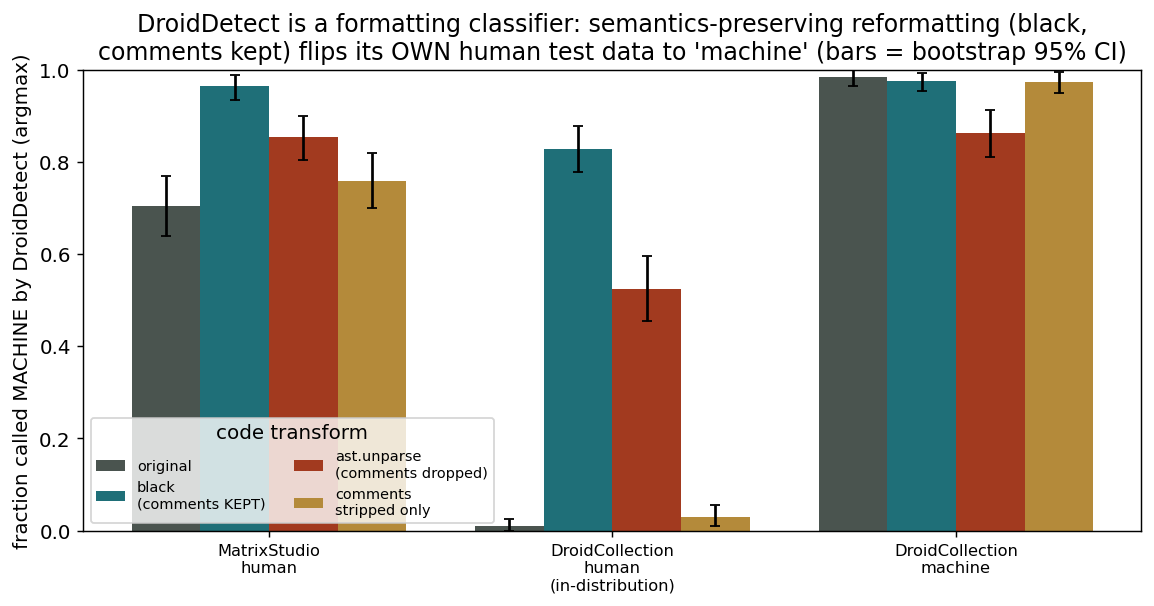
\includegraphics[width=0.95\linewidth]{fig7_format_ablation.png}
\caption{Semantics-preserving reformatting flips DroidDetect's verdict on the authors'
\emph{own} human test data. Running it through \texttt{black} (comments kept) raises the
``machine'' rate from \resAblDcHumanOrig{} to \resAblDcHumanBlack{} (\texttt{ast.unparse}:
\resAblDcHumanCanon{}); comment-stripping alone barely moves it (\resAblDcHumanStrip{}); already
auto-formatted \emph{machine} code is essentially unchanged. Identifiers and literals are preserved
exactly, so the operative signal is layout/quote/wrap style.}
\label{fig:ablation}
\end{figure}

\paragraph{Why---a training-data formatting confound (suggestive).} This shortcut is surprising,
since humans run \texttt{black} too. The likely origin is in the data: the two training classes
differ in formatting cleanliness. As a coarse proxy, a fraction \resFmtHumanAlreadyBlack{} of
\emph{human} DroidCollection Python is already \texttt{black}-compliant versus
\resFmtMachineAlreadyBlack{} of \emph{machine} Python (mean similarity-to-\texttt{black}
\resFmtHumanBlackSim{} vs \resFmtMachineBlackSim{})---a roughly threefold gap. Machine code is born clean---freshly generated
by LLMs that emit canonical PEP8-ish layout---while human code carries its original formatting, so
a loss-minimizing classifier can exploit this almost-free cue instead of learning authorship. We
flag this metric as \emph{suggestive rather than decisive}: a string-similarity-to-\texttt{black}
ratio is sensitive to code length and content, and we did not length-control it, so the magnitude
of the 15-vs-44\% gap should not be over-read. The causal claim of the headline rests on the
\emph{within-corpus} ablation (Fig.~\ref{fig:ablation}), where source is held fixed; the data
statistic only proposes a mechanism. Because real human code is routinely auto-formatted, the cue
is invalid at deployment regardless of its exact training-set magnitude.

\subsection{The confound is family-wide, not a single checkpoint}
\label{sec:family}
A web audit found no clean independent out-of-the-box trained \emph{code} detector to compare
against, so we tested all \resSibFamilyN{} published DroidDetect siblings---different sizes
(ModernBERT base/large) and granularities (2- and 4-class)---through the same probe
(Table~\ref{tab:family}). The black-flip reproduces on every one: in-distribution human code goes
from at most \resSibFamilyHumanOrigMax{} ``machine'' to between \resSibFamilyHumanBlackMin{} and
\resSibFamilyHumanBlackMax{}. Scaling to the Large encoder does \emph{not} fix it. This rules out
``a quirk of one checkpoint'' and ``the small model is undertrained,'' and is consistent with a
cause in the shared training data. It does \emph{not}, by itself, prove the cause is the data
rather than the shared recipe, because all siblings share authors, architecture family, and
DroidCollection; the decisive test---an independent architecture trained on the same data---is
left to future work (Sec.~\ref{sec:limitations}).

\begin{table}[h]\centering
\begin{tabular}{lcccccc}
\toprule
Detector & classes & DC-human orig.\ & DC-human \texttt{black} & DC-machine & MS-human & legendary\\
\midrule
Base-Binary  & \resSibBaseBinaryNClasses{}  & \resSibBaseBinaryHumanOrig{}  & \textbf{\resSibBaseBinaryHumanBlack{}}  & \resSibBaseBinaryMachine{}  & \resSibBaseBinaryMsHuman{}  & \resSibBaseBinaryLegAll{}\\
Base         & \resSibBaseFourNClasses{}    & \resSibBaseFourHumanOrig{}    & \textbf{\resSibBaseFourHumanBlack{}}    & \resSibBaseFourMachine{}    & \resSibBaseFourMsHuman{}    & \resSibBaseFourLegAll{}\\
Large-Binary & \resSibLargeBinaryNClasses{} & \resSibLargeBinaryHumanOrig{} & \textbf{\resSibLargeBinaryHumanBlack{}} & \resSibLargeBinaryMachine{} & \resSibLargeBinaryMsHuman{} & \resSibLargeBinaryLegAll{}\\
\bottomrule
\end{tabular}
\caption{Fraction called ``machine'' (native argmax) across the DroidDetect family. Every sibling
flips its own in-distribution human code from near zero to a large majority under \texttt{black}
(bold), over-flags cross-source human code (MS), and flags provably-human pre-LLM elite code
(legendary). Scaling to Large does not help.}
\label{tab:family}
\end{table}

\subsection{The skill confound is a (bounded) null on the competitive-skill axis}
We find no evidence that competitive-programming skill confounds detection---but this is a
\emph{null}, and we are explicit about its limits. The skill-matched vs.\ mismatched AUROC gap is
small for all detectors (Table~\ref{tab:delta}, Fig.~\ref{fig:delta}):
$\Delta_{\text{confound}}=\resDeltaDroidDetect{}$ (CI $[\resDeltaCIloDroidDetect{},\resDeltaCIhiDroidDetect{}]$)
for DroidDetect, \resDeltaFastDetectGPT{} and \resDeltaBinoculars{} for the statistical detectors.
The CI bounds the confound below $\approx$\,\resDeltaCIhiDroidDetect{} AUROC---we can rule out a
\emph{large} skill confound on this axis, not assert a true zero. Two caveats temper even this:
(i) the matched/mismatched AUROCs themselves are mediocre (\resAurocMatchedDroidDetect{} /
\resAurocMismatchedDroidDetect{} for DroidDetect; \resAurocMatchedFastDetectGPT{} /
\resAurocMatchedBinoculars{} for the statistical detectors), so $\Delta\approx0$ partly reflects a
\emph{floor}---there is little performance left to collapse on terse competitive code; (ii) human
code is accepted-only, a selection collider (rating$\to$accept$\leftarrow$difficulty).

Within-species slopes (Table~\ref{tab:slopes}, Fig.~\ref{fig:slopes}) point, if anything,
\emph{against} a skill-tracking account: the human slope is negative for DroidDetect
($\resHumanSlopeDroidDetect{}$, CI $[\resHumanSlopeLoDroidDetect{},\resHumanSlopeHiDroidDetect{}]$)
and Fast-DetectGPT ($\resHumanSlopeFastDetectGPT{}$), and null for Binoculars
($\resHumanSlopeBinoculars{}$). We do \emph{not} interpret the negative sign as ``skill inverts'':
the accepted-only collider can manufacture a negative slope by selecting atypical (terse,
hyper-optimized) hard-problem solutions. The defensible reading is only that higher
\skillaxis{} skill is \emph{not} scored more AI-like, contrary to H$_\text{skill}$.

\begin{table}[h]\centering
\begin{tabular}{llrr}
\toprule
Detector & Family & Human slope (hard$-$easy) & LLM slope (novice$\to$expert)\\
\midrule
DroidDetect    & trained     & \resHumanSlopeDroidDetect{}    & \resLlmSlopeDroidDetect{}\\
Fast-DetectGPT & statistical & \resHumanSlopeFastDetectGPT{}  & \resLlmSlopeFastDetectGPT{}\\
Binoculars     & statistical & \resHumanSlopeBinoculars{}     & \resLlmSlopeBinoculars{}\\
\bottomrule
\end{tabular}
\caption{Within-species skill slopes (z-scored detector score). Positive${}={}$skill-tracking.}
\label{tab:slopes}
\end{table}

\begin{table}[h]\centering
\begin{tabular}{llrrr}
\toprule
Detector & Family & AUROC matched & AUROC mismatched & $\Delta_{\text{confound}}$\\
\midrule
DroidDetect    & trained     & \resAurocMatchedDroidDetect{}    & \resAurocMismatchedDroidDetect{}    & \resDeltaDroidDetect{}\\
Fast-DetectGPT & statistical & \resAurocMatchedFastDetectGPT{}  & \resAurocMismatchedFastDetectGPT{}  & \resDeltaFastDetectGPT{}\\
Binoculars     & statistical & \resAurocMatchedBinoculars{}     & \resAurocMismatchedBinoculars{}     & \resDeltaBinoculars{}\\
\bottomrule
\end{tabular}
\caption{AUROC by skill cell and $\Delta_{\text{confound}}$ (cluster-bootstrap over problems).}
\label{tab:delta}
\end{table}

\begin{figure}[h]\centering
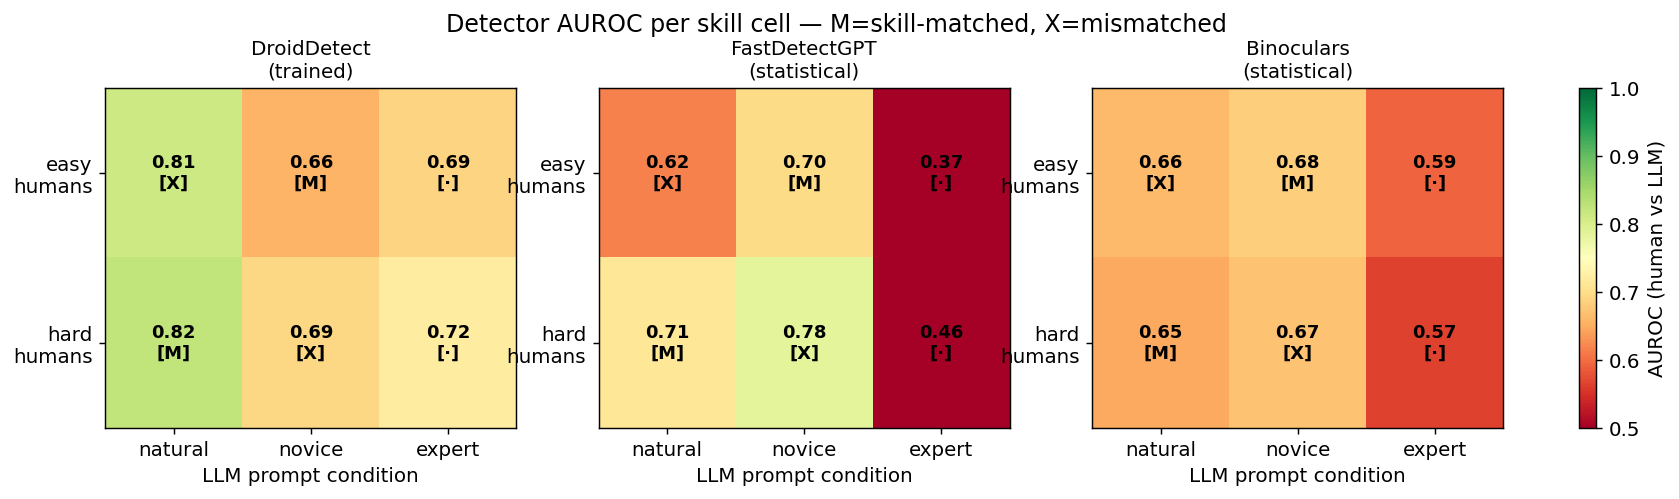
\includegraphics[width=\linewidth]{fig1_auroc_heatmaps.png}
\caption{AUROC per (detector, difficulty band, prompt condition). M${}={}$skill-matched,
X${}={}$mismatched.}
\label{fig:heat}
\end{figure}

\begin{figure}[h]\centering
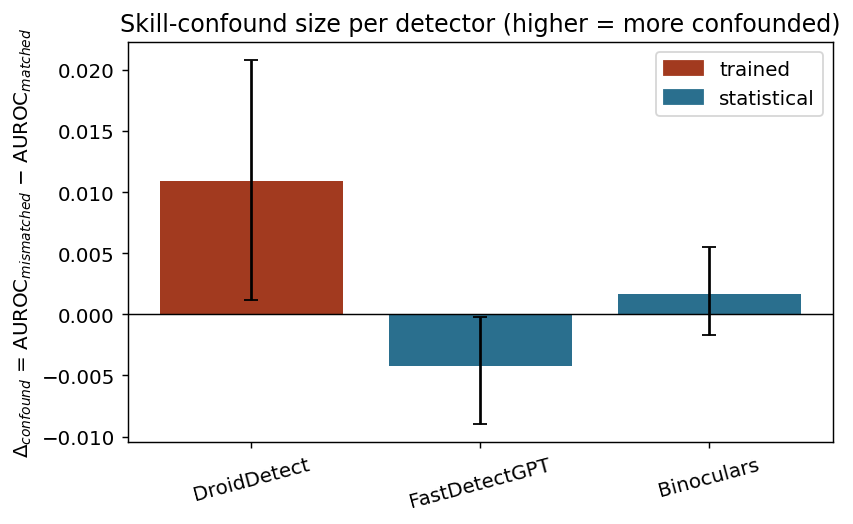
\includegraphics[width=0.7\linewidth]{fig2_delta_confound.png}
\caption{$\Delta_{\text{confound}}$ per detector with cluster-bootstrap 95\% CIs; all intervals
sit near zero, bounding any competitive-skill confound to be small on this axis.}
\label{fig:delta}
\end{figure}

\subsection{Cross-source generalization failure (the dominant effect)}
DroidDetect is a softmax classifier whose actual prediction is the \emph{argmax} over
$\{$human, machine$\}$, with no tunable threshold; we report it at that native operating point and
measure its \emph{true} false-positive rate on ordinary human code. On clean human Codeforces
Python from a \emph{different} source~\citep{matrixstudio2024codeforces} the FPR explodes from
\resDroidInDistHumanFPR{} (in-distribution) to \resDroidArgmaxCfHumanFPR{}: that fraction of
\emph{ordinary} human solutions are called AI (vs.\ \resDroidArgmaxCfLlm{} of actual Codeforces LLM
code---so it barely separates the two out of distribution). On the provably-human pre-LLM elite
corpus the rate is \resDroidArgmaxLegendary{}---essentially the \emph{same} as its cross-source
human FPR (\resDroidArgmaxCfHumanFPR{}). We therefore read the legendary result as the \emph{same}
domain-shift/formatting over-flagging affecting all human code here, \textbf{not} a distinct
``elite code looks AI'' effect. Per-author rates do vary (CPython \resDroidArgmaxCPythonCore{},
Hipp \resDroidArgmaxDRichardHipp{}, antirez \resDroidArgmaxSalvatoreSanfilippo{}, Torvalds'
original \texttt{git} \resDroidArgmaxLinusTorvalds{}), but with as few as $15$ samples per author
and Torvalds sitting \emph{below} the ordinary-human baseline, we do not interpret an ordering. The
statistical detectors, shown at a fixed 5\%-FPR operating point for comparability, flag the same
code far less (Fast-DetectGPT \resLegFlagFastDetectGPT{}, Binoculars \resLegFlagBinoculars{})---but
recall they are near-random as detectors on this domain, so this is robustness, not usefulness.

\begin{figure}[h]\centering
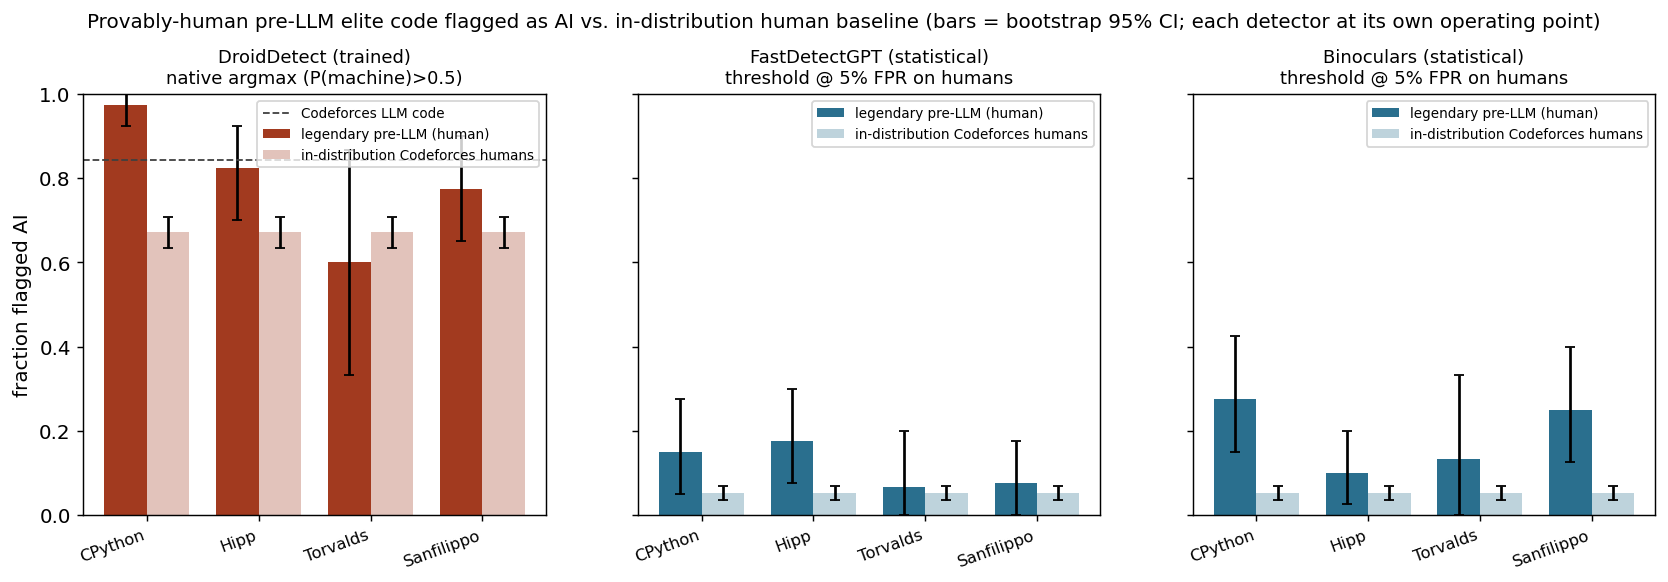
\includegraphics[width=0.8\linewidth]{fig4_legendary_flag_rates.png}
\caption{Provably-human pre-LLM elite code flagged as AI (solid), with the in-distribution
ordinary-human baseline beside each (semitransparent); bootstrap 95\% CIs. DroidDetect is
shown at its native argmax operating point (baseline${}={}$its true cross-source human FPR,
\resDroidArgmaxCfHumanFPR{}); the statistical detectors at a fixed 5\%-FPR point.}
\label{fig:legendary}
\end{figure}

\subsection{Mechanism and confirmatory checks}
Surface style features explain $R^2=\resStyleRsqDroidDetect{}$ of DroidDetect's score and
$\resStyleRsqFastDetectGPT{}$ of Fast-DetectGPT's---style matters but does not fully
account for the trained detector. On the harder Codeforces problems human code is in fact
\emph{more} idiomatic (type-hint rate \resStyleHasTypeHintsEasy{}${}\to{}$\resStyleHasTypeHintsHard{},
Fig.~\ref{fig:diffstyle}), which makes the negative human slope notable: more idiomatic
\emph{competitive} code is still not read as more AI.

A cohort using real \emph{author} Elo (AtCoder~\citep{atcoder}; low band $n=\resAtNLowSkill{}$
mean Elo \resAtRatingLowSkill{}, high band $n=\resAtNHighSkill{}$ mean Elo \resAtRatingHighSkill{})
is directionally consistent---the high$-$low score gap is negative for all detectors
(e.g.\ DroidDetect \resAtHiLoDroidDetect{} SD, Fig.~\ref{fig:atcoder})---but the high band is far
too thin ($n=\resAtNHighSkill{}$) for its slope CI to exclude zero, so we treat it as suggestive
only, not as confirmation.

\begin{figure}[h]\centering
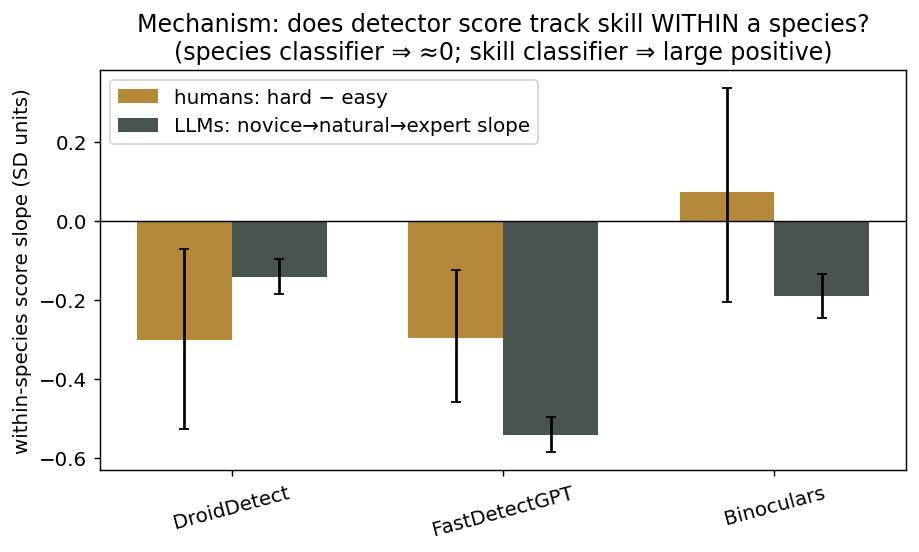
\includegraphics[width=0.7\linewidth]{fig3_within_species_slopes.png}
\caption{Within-species slopes: detector score vs.\ skill, per species.}
\label{fig:slopes}
\end{figure}

\begin{figure}[h]\centering
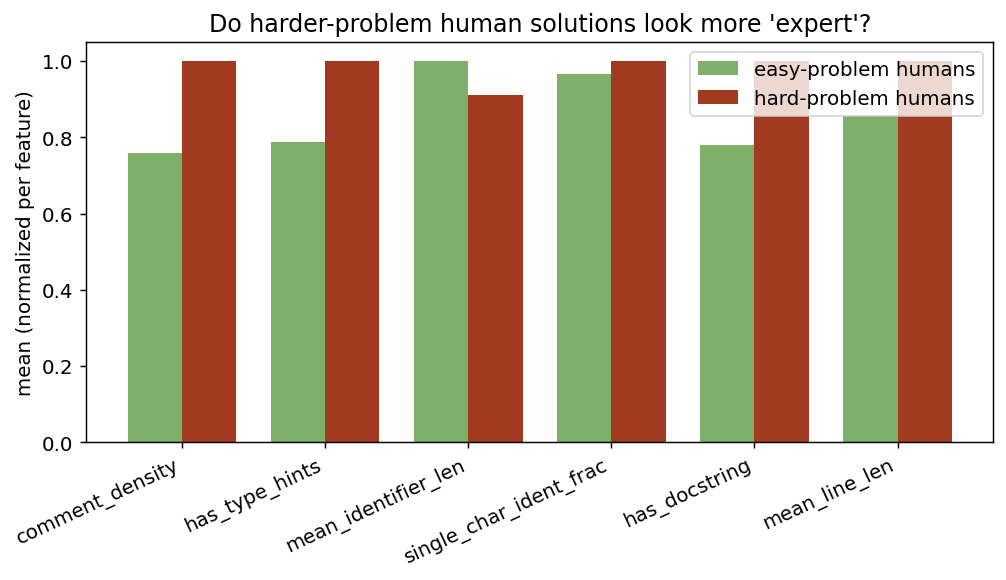
\includegraphics[width=0.7\linewidth]{fig5_difficulty_to_style.png}
\caption{Human code style vs.\ problem difficulty: harder problems draw \emph{more} idiomatic
code (higher type-hint rate), so the difficulty proxy is stylistically inverted relative to the
``senior-engineer'' register that motivates H$_\text{skill}$.}
\label{fig:diffstyle}
\end{figure}

\begin{figure}[h]\centering
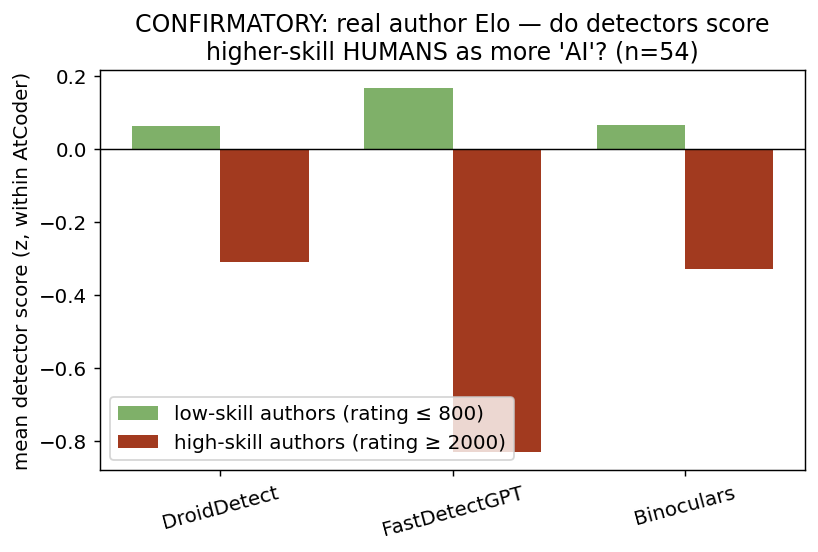
\includegraphics[width=0.7\linewidth]{fig6_atcoder_author_skill.png}
\caption{AtCoder author-Elo cohort: detector score vs.\ real author rating. Directionally
consistent with the difficulty-axis null but underpowered (high band $n=\resAtNHighSkill{}$).}
\label{fig:atcoder}
\end{figure}

\section{Limitations}
\label{sec:limitations}
\begin{itemize}
  \item \textbf{Single-corpus red-team.} Every trained detector here is the DroidDetect family:
        same authors, same DroidCollection training data, same ModernBERT backbone. We show the
        formatting shortcut is family-wide and not a single-checkpoint quirk, but whether it
        generalizes beyond this data \emph{recipe} is untested. The decisive experiment---training
        an \emph{independent} architecture (e.g.\ CodeBERT/RoBERTa) on DroidCollection and
        re-running the ablation---would separate ``the data is confounded'' from ``the
        DroidDetect recipe is confounded'' and also rule out a ModernBERT-tokenizer artifact; it is
        proposed, not run.
  \item \textbf{Formatting metric is suggestive.} The human-vs-machine black-compliance gap
        (\resFmtHumanAlreadyBlack{} vs \resFmtMachineAlreadyBlack{}) uses an un-length-controlled
        string-similarity ratio; it motivates the mechanism but is not the
        load-bearing evidence (the within-corpus ablation is).
  \item \textbf{Problem difficulty / rating $\ne$ idiomatic-code skill}, and the proxy is
        stylistically inverted; the skill result is a bounded null, not a true zero.
  \item \textbf{Accepted-only human code} is a selection collider; LLM code is unfiltered---asymmetric.
  \item \textbf{Small LLM panel} (gemma-2-2b, Qwen2.5-3B, gpt-5.4-nano) and \textbf{thin AtCoder
        high-skill band} ($n=\resAtNHighSkill{}$); preliminary $n$ throughout.
  \item \textbf{MatrixStudio is a different human source} than DroidCollection's training data; we
        cannot fully separate ``source shift'' from ``formatting'' for the cross-source FPR, though
        the within-corpus ablation isolates formatting and the pre-LLM legendary probe is the
        contamination-free anchor.
\end{itemize}

\section{Reproducibility}
All numbers in this report are emitted by scripts into \texttt{paper/macros.tex} and referenced by
name; all bibliography metadata is fetched from arXiv into \texttt{paper/refs.bib}. The full pipeline
reproduces end-to-end via \texttt{./run\_pipeline.sh} (single GPU). Detector checkpoints are the
released \texttt{project-droid/DroidDetect-*} weights, loaded verbatim from their model card; the
zero-shot detectors use vendored upstream implementations. Generation uses HuggingFace
\texttt{transformers} (the local vLLM build is ABI-incompatible), and \texttt{black} is invoked
through \texttt{uvx} so the shared environment is untouched. Seeds and model revisions are recorded
in the repository.

\section{Conclusion}
The headline is mechanistic and cautionary: the strongest off-the-shelf trained code detector we
could obtain has its decision \textbf{gated by formatting}. Faithfully loaded (AUROC
\resDroidInDistAUROC{}, \resDroidInDistHumanFPR{} FPR on the authors' own data), it nonetheless
flips from \resAblDcHumanOrig{} to \resAblDcHumanBlack{} ``machine'' on that \emph{same} human data
under a semantics-preserving reformatting, and the flip reproduces across every sibling in the
family. That dependence explains the rest: \resDroidArgmaxCfHumanFPR{} of ordinary human Codeforces
code from a different scrape, and \resDroidArgmaxLegendary{} of provably-human pre-LLM elite code,
are flagged not because they are AI-like or expert but because their formatting differs from the
training-human formatting. Secondarily, ``does detection reduce to \emph{skill}?''---not to
competitive-programming skill, where the confound is a bounded null. The zero-shot statistical
detectors do not collapse under formatting, but are near-random here, so no detector we tested is
deployable on this domain; they fail differently. The deployment implication is stark and is a
\emph{false-positive} risk, not an evasion trick: a student or developer whose only ``offense'' is
running an autoformatter can be flagged as AI by an integrity tool of this kind, and the tool's
reported accuracy---all i.i.d., with no fixed-FPR or calibration reporting---hides this. Clean
follow-ups: an independent-architecture replication of the ablation, evaluation under
format-normalization and across held-out human \emph{sources}, and calibrated fixed-FPR operating
points.

\bibliographystyle{plainnat}
\bibliography{refs}

\end{document}
